\subsection{E7 --- Objection 2: is the quality proxy real?}
\label{sec:real}
\textbf{Question.} Everything so far scores quality with $\epsilon\times$(attention mass served from \warm{}). Does a policy that the proxy ranks better also change the real model's output less when INT4 is actually applied? \textbf{Setup.} For each of the 42 images, we replay each policy's placement on the real SmolVLM-256M. The simulator logs, for every decode step, which (token, layer) entries are in \warm{}; the model is then teacher-forced on its own full-precision 64-token generation, and at step $t$ the cached K and V of exactly those entries are replaced by their INT4 round trip (per-token asymmetric min-max, groups of 32). We measure the KL divergence $\mathrm{KL}(p_{\text{full}}\,\|\,p_{\text{policy}})$ of the next-token distribution (mean over the 64 steps) and top-1 agreement with the full-precision model. The replay reproduces the saved generation on all 42 images. Four placements are compared: static modality, the dynamic policy (selected thresholds 8/0.4), \emph{random placement with the same number of INT4 entries at every step as the dynamic policy} (a control for \emph{which} entries are demoted), and everything in INT4.

\begin{figure}[t]
\centering
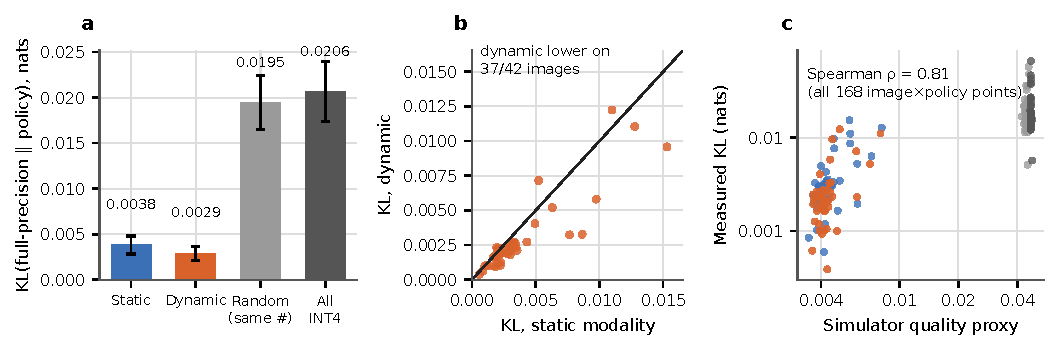
\includegraphics[width=\linewidth]{figs/fig_real_output.pdf}
\caption{E7: real output change under INT4 placement, 42 images, SmolVLM-256M. (a) Mean KL to the full-precision model (95\% CIs). (b) Dynamic vs static per image: points below the diagonal favour the dynamic policy. (c) The simulator's quality proxy against measured KL for all 168 (image, policy) points.}
\label{fig:real}
\end{figure}

\begin{table}[t]
\centering\small
\caption{E7: measured effect of INT4 placement on the next-token distribution (mean over 42 images). Fraction of entries in INT4 is the mean over steps.}
\label{tab:e7}
\begin{tabular}{lcccc}
\toprule
Placement & INT4 entries & KL (nats) & Top-1 agreement & Proxy $\epsilon\!\cdot\!$mass\\
\midrule
Static modality               & 91.8\% & 0.00382 & 0.976 & 0.0045\\
Dynamic (ours)                & 94.9\% & \textbf{0.00291} & 0.977 & 0.0044\\
Random, same INT4 count       & 94.9\% & 0.01946 & 0.930 & 0.0445\\
All INT4                      & 100\%  & 0.02064 & 0.929 & 0.0468\\
\bottomrule
\end{tabular}
\end{table}

\textbf{Finding 1: the policy picks the right entries.} The dynamic policy places \emph{more} entries in INT4 than static modality (94.9\% vs 91.8\%) and still changes the output distribution \textbf{21.8\% less} (per-image mean, 95\% CI $[15.3,28.1]\%$; lower on 37 of 42 images: 22/24 natural, 9/10 chart, 6/8 document). Random placement with the same INT4 count is \textbf{9.4$\times$} worse than the dynamic policy ($[7.8,11.1]\times$; worse on all 42 images) and indistinguishable from putting everything in INT4. The energy saving of E5 is therefore not obtained by demoting entries at random, and the entries the policy keeps in \hot{} are the ones the real model is sensitive to.

\textbf{Finding 2: the proxy is a usable but conservative guide.} Across all 168 points the proxy and the measured KL are strongly rank-correlated (Spearman $\rho{=}0.81$; Pearson on log scale 0.88), mostly because the proxy separates policies that demote important entries from those that do not (Fig.~\ref{fig:real}c). Within the static/dynamic pair the correlation is weaker ($\rho{=}0.49$), the proxy's per-image sign of the dynamic-vs-static difference matches the measured one on 29 of 42 images, and it \emph{understates} the advantage: the proxy predicts $-2.5\%$, the measurement $-21.8\%$. Top-1 agreement does not separate dynamic from static (difference $+0.1$ points, CI includes 0). \textbf{Caveats.} The effects of INT4 on this small model are small in absolute terms (even all-INT4 keeps 93\% top-1 agreement over 64 teacher-forced steps), so E7 validates the \emph{ordering and mechanism} rather than a task-accuracy claim, covers one model and the single INT4 scheme measured in Sec.~3.2, and uses KL as the quality measure, not a benchmark score.
